% !TEX root = ../../document.tex

\documentclass{subfiles}

\begin{document}

  \chapter{Algoritmos aplicados a Grafos}
  \label{chap:graphs}

    \section{Introducción}
    \label{sec:graphs_intro}

      \paragraph{}
      [TODO]

    \section{Definición Formal}
    \label{sec:graph_formalism}

      \paragraph{}
      En esta sección se describen los conceptos básicos necesarios para entender el estudio de problemas basados en \emph{Grafos}. Para la descripción formal sobre dichas estructuras se han utilizado las notas de clase de la asignatura de \emph{Matemática Discreta} \cite{matematicaDiscreta2016notes} impartida en la \emph{Universidad de Valladolid} así como las de la asignatura equivalente (\emph{Discrete Mathematics CS 202} \cite{aspnes2013notes}) impartida por \emph{Aspnes} en la \emph{Universidad de Yale}.

      \paragraph{}
      La \textbf{Teoría de Grafos} (\emph{Graph Theory}) es la disciplina encargada del estudio de estructuras compuestas por vértices y aristas desde una persepectiva matemática. Los vértices representan objetos mientras que las aristas se corresponden con la modelación de las relaciones entre estos. Un grafo $G$ se define por tanto como la tupla del conjunto de vértices $V = \{ v_1, _2, ..., v_n \}$ y las aristas $E = \{ e_1, e_2, ..., e_m \}$, de tal manera que $e_j = (v_{i_1}, v_{i_2})$ representa el arista que conecta el vértice $v_{i_1}$ con $v_{i_2}$. Nótese por tanto que el grafo está compuesto por $n$ vértices y $m$ aristas. El grafo $G$ se puede modelizar por tanto como $G = (V, E)$. En la figura \ref{img:graph_example} se muestra una representación gráfica de un determinado grafo no dirigido compuesto por $6$ vértices y $7$ aristas.

      \begin{figure}
        \centering
        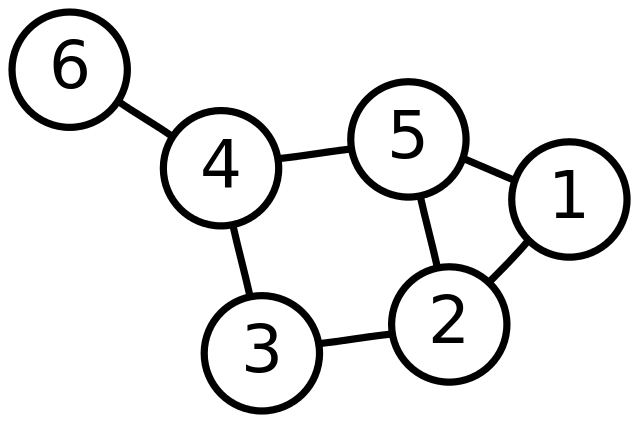
\includegraphics[width=0.4\textwidth]{graph-example}
        \caption{Ejemplo de \emph{Grafo No Dirigido}. (Extraido de \cite{wiki:Graph_(discrete_mathematics)})}
        \label{img:graph_example}
      \end{figure}

      \paragraph{}
      Aquellos grafos para los cuales la arista $e_j$ representa los dos sentidos de la relación, es decir, $v_{i_1}$ está relacionado con $v_{i_2}$ y $v_{i_2}$ está relacionado con $v_{i_1}$ se denominan \emph{Grafos no nirigidos}, mientras que en los casos en que esta relación no es recíproca se habla de \emph{Grafos dirigidos}. Cuando cada arista $e_j$ tiene asociado un determinado peso $w_j \in W =  \{ w_1, w_2, ..., w_m\}$ se dice entonces que $G$ es un \emph{grafo ponderado} mientras que cuando se presupone que todas las aristas tienen el mismo peso se omite dicha notación.

      \paragraph{}
      Cuando un vértice denominado $v_{i_1} \in V$ está directamente relacionado con otro denominado $v_{i_2} \in V$, es decir, existe una arista $e_j \in E$ que los conecta ($e_j = (v_{i_1}, v_{i_2})$) se dice que son $e_j$ es \emph{incidente} de dichos vértices. De la misma manera se dice que $v_{i_1}$ y $v_{i_2}$ son \emph{adjacentes} entre sí.

      \paragraph{}
      Respecto del número de aristas incidentes sobre cada vértice, se denomina \emph{grado} al cardinal de estas, diferenciando en los grafos no dirigidos entre \emph{in-grado} a las de destino y \emph{out-grado} a las de salida. Se utiliza la notación $d(v_i)$ para referirse al grado del vértice i-ésimo, $d^+(v_i)$ al \emph{in-grado} y $d^-(v_i)$ al \emph{out-grado} de dicho vértice. Nótese que se cumple la siguiente propiedad: $d(v_i) = d^+(v_i) + d^-(v_i)$.


      \paragraph{}
      Un \emph{camino} es un conjunto de aristas $P_p = \{ e_{k_1}, e_{k_2}, ..., e_{k_p}\}$ tales que la arista k-ésima tiene como vércice de destino el mísmo que utiliza la $k+1$ como vércice origen. Nótese que el valor $p$ indica la \emph{longitud} del camino. Cuando el vértice de destino de la arista $e_{k_p}$ es el mismo que el de origen de $e_{k_1}$ se denomina \emph{ciclo} y se denomina $C_p$.

      \paragraph{}
      Se denomina $K_n$ al grafo compuesto por $n$ vértices y $n*(n-1)$ aristas, de tal manera que estas conectan cada vértice con todos los demás. Los grafos que cumplen esta propiedad se denominan grafos completos de grado $n$. Nótese que este número se reduce a la mitad en el caso de los grafos no dirigidos.

      \paragraph{}
      Cuando en un grafo al estudiar la estructura de un grafo, se comprueba que el conjunto de vértices puede dividirse en dos subconjuntos disjuntos $V_1$ y $V_2$ de tal manera que para todas las aristas $e_j = (v_{i_1}, v_{i_2})$ el vértice $v_{i_1}$ se encuentra en el subconjunto $V_1$ y el vértice $v_{i_2}$ se encuentra en el subconjunto $V_2$, entonces se habla de un \emph{Grafo Bipartito}. Un ejemplo de esta situación se muestra en la figura \ref{img:bipartite_graph_example}. Nótese que el concepto de grafo bipartito puede extenderse fácilmente a más de dos subconjuntos, denominandose entonces \emph{Grafo k-partito}. Estos grafos tienen son de gran utilidad para modelizar algunos problemas tales como \emph{Netflix} para los cuales $V_1$ puede estar formado por el conjunto de usuarios mientras que $V_2$ representa el contenido multimendia. Por tanto, cada arista representa las visualizaciones de los usuarios.

      \begin{figure}
        \centering
        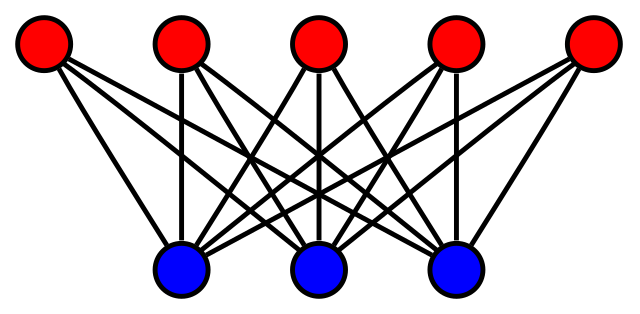
\includegraphics[width=0.4\textwidth]{bipartite-graph-example}
        \caption{Ejemplo de \emph{Grafo Bipartito}. (Extraido de \cite{wiki:Graph_(discrete_mathematics)})}
        \label{img:bipartite_graph_example}
      \end{figure}

      \paragraph{}
      Un \emph{subgrafo} $H$ es el grafo compuesto por un subconjunto de vectores y aristas del grafo $G$. Nótese que en el caso de que eliminen vértices, es necesario eliminar también todas sus aristas incidentes. Esto se puede indicar de manera matemática de la siguiente forma: $H \subseteq G$ por lo que $H_V \subseteq G_V$ y $H_E \subseteq G_E$.

      \paragraph{}
      Desde el punto de vista de las transformaciones que se pueden realizar sobre grafos, se denomina \emph{isomorfismo} a una transformación biyectiva sobre el grafo $G =(V_G, E_G)$ al grafo $H = (V_H, E_H)$ que se realiza sobre los vértices de manera que $f: V_G \rightarrow V_H$ y por cada arista $(e_1, e_2) \in E_G$, entonces $(f(e_1), f(e_2)) \in E_H$ de tal manera que la estructura de $G$ se conserva en $H$. Entonces se dice que $G$ y $H$ son isomorfos entre si. Si se modifica la condición de biyectividad del \emph{isomorfismo} y tan solo se requiere la propiedad de inyectividad entonces se habla de \emph{homomorfismo}. Por tanto, esto puede ser visto como una transformación en la cual no se mantiene completamente la estructura, entonces $H$ ya no es equivalente a $G$, sino que es un \emph{subgrafo} de este.

      \paragraph{}
      Las transformaciones \emph{homomórficas} son interesantes desde el punto de vista del tratamiento de grafos de tamaño masivo, dado que a partir de estas se trata de reducir la complejidad cuando el tamaño de estos los hace intratables. Por lo tanto, interesa conseguir \emph{homomorfismos} que reduzcan el tamaño del grafo, pero que traten de mantener su estructura lo más semejante posible. Destacan transformaciones conocidas como \emph{Spanners} (Sección \ref{sec:spanners}) y \emph{Sparsifiers} (Sección \ref{sec:sparsifiers}).

      \subsection{Métodos de Representación}
      \label{sec:laplacian_matrix}

        \paragraph{}
        Existen diversas alternativas de representación de grafos, las cuales presentan ventajas e inconvenientes tanto a nivel de espacio como de tiempo de acceso. Dichas estrategias se escogen teniendo en cuenta la estructura del grafo. En esta sección se habla de matrices de adyacencia y de listas de adyacencia.

        \subsubsection{Matriz de Adyacencia}
        \label{sec:adjacency_matrix}

          \paragraph{}
          Se denomina matriz de adyacencia $A$ del grafo $G = (V,E)$ compuesto por $n=|V|$ vértices, $m=|E|$ aristas y $w_k \in W$ el peso de la arista $e_k$, a una matriz de tamaño $n*n$ construida tal y como se indica en la ecuación \eqref{eq:adjacency_matrix}. Nótese que esta definición es válida tanto para grafos ponderados como para no ponderados suponiendo que $w_k = 1, k \in [1, m]$.

          \begin{equation}
          \label{eq:adjacency_matrix}
            A_{i,j} =
              \begin{cases}
                w_k,  & (v_i, v_j) = e_k \in E\\
                0,    &\text{en otro caso}
              \end{cases}
          \end{equation}

          \paragraph{}
          Esta estrategia de representación es apropiada cuando se trabaja sobre grafos altamente conexos (con un gran número de aristas), ya que el número de posiciones nulas en la matriz es reducido y la estructura indexada matricial proporciona un tiempo de acceso de $O(1)$. Sin embargo se requiere de $O(n^2)$ para almacenar dicha matriz, algo admisible cuando $n^2 \approx m$ para los cuales esta representación se acerca al óptimo a nivel de espacio.

        \subsubsection{Lista de Adyacencia}
        \label{sec:adjacency_list}

          \paragraph{}
          La alternativa a la codificación del grafo como una matriz de adyacencia se conoce como \emph{lista de adyacencia}. En este caso se mantiene una lista (posiblemente ordenada u otras estrategias más estructuradas como listas enlazadas para reducir los tiempos de acceso) compuesta por el conjunto de aristas $E$. Nótese por tanto que en este caso la codificación es óptima a nivel de espacio $O(m)$, no existiendo una estrategia de representación exacta que pueda almacenar la estructura del mismo utilizando un tamaño menor. Sin embargo, tal y como se puede intuir, el tiempo de acceso es de $O(m)$ en el peor caso, para lo cual se puede tratar de mejorar el caso promedio manteniendo una lista ordenada. Esta solución es apropiada para grafos dispersos (aquellos en que $n \ll m$).

        \paragraph{}
        En la práctica, cuando se trabaja con grafos de tamaño masivo, es muy común que estos sean muy dispersos. Algunos ejemplos de ellos son el \emph{grafo de la web} (grafo dirigido), en el cual cada vértice representa sitio web y cada arista un enlace hacia otro sitio web. Es fácil comprobar que este grafo es altamente disperso ya que es muy poco probable que un sitio web contenga enlaces al resto de sitios de la red cuando se habla de millones de vértices. Algo similar ocurre en el caso de redes sociales como \emph{Facebook} (grafo no dirigido debido a relaciones de amistad) o \emph{Twitter} (grafo dirigido debido a relaciones seguimiento). Por tanto, la representación mediante listas de adyacencia es una herramienta útil a nivel conceptual pero en la práctica se utilizan otras alternativas por la inviabilidad derivada del gran coste espacial en la representación.


        \subsubsection{Matrix Laplaciana}
        \label{sec:laplacian_matrix}

          \paragraph{}
          La \emph{matriz laplaciana} consiste en una estrategia de representación de grafos que cumple importantes propiedades a partir de las cuales se facilita en gran medida la resolución de un gran número de problemas sobre grafos.

          \paragraph{}
          [TODO ]

          \paragraph{}
          [TODO ]

          \paragraph{}
          [TODO ]

    \section{Modelo en Semi-Streaming}
    \label{sec:semi_streaming_model}

      \paragraph{}
      Al igual que en el caso de conjuntos de datos de carácter numérico o categoríco, en el modelo de grafos, también es necesario hacer frente al elevado tamaño del problema mediante nuevos paradigmas de diseño de algoritmos. El \emph{modelo en streaming}, del cual se habló en la sección \ref{sec:streaming_model} es una buena alternativa para tratar de agilizar la búsqueda de soluciones que varían con respecto del tiempo, además de trabajar sobre un espacio reducido. Tal y como se indicó anteriormente, esta estrategia permite reducir el número de acceso sobre el dispositivo de almacenamiento tratando de trabajar únicamente con los estimadores que se mantienen en la memoria del sistema, cuyo tiempo de acceso es mucho más rápido.

      \paragraph{}
      Sin embargo, en el caso de los problemas referidos a grafos, este modelo presenta mayores dificultades, tanto a nivel de espacio como del número de accesos sobre el stream de datos. Por lo tanto, se han definido variaciones sobre el \emph{modelo en streaming} original para tratar de hacer frente a los requisitos característicos de este tipo de problemas. En los artículos \emph{On graph problems in a semi-streaming model} \cite{feigenbaum2005graph} y \emph{Analyzing graph structure via linear measurements} \cite{ahn2012analyzing} los autores describen dicho modelo, al cual denominan \textbf{Modelo en Semi-Streaming}.

      \paragraph{}
      Este se corresponde con una relajación del \emph{modelo en streaming} estándar, el cual permite mayor libertad tanto a nivel de espacio como de pasadas permitidas sobre el stream de datos. Por esta razón, cuando el número de pasadas  $k$ es superior a 1 ($k > 1$), entonces ya no es posible su uso en entornos en que se requiere que el procesamiento de la información así como las respuestas sean obtenidas en tiempo real, algo que si sucedía en el caso del \emph{modelo en streaming} definido anteriormente. Por lo tanto, el \emph{modelo en semi-streaming} se presenta como una estrategia de diseño de algoritmos que trata de obtener estimaciones sobre grafos en un espacio reducido y con un buen planteamiento a nivel de accesos a disco cuando el grafo completo no puede mantenerse en la memoria del sistema de manera completa.

      \paragraph{}
      El \emph{modelo en semi-streaming} impone la forma en que el grafo es suministrado bajo la idea de stream de datos. Esta se describe a continuación: Sea $G = (V, E)$ un grafo dirigido (su adaptación al caso de grafos dirigidos es trivial) compuesto por $n = |V|$ vértices y un número indeterminado de arístas desde el punto de vista del algoritmo que procesará el stream. Se presupone que se conoce \emph{a-priori} el número de vértices que forman el grafo, mientras que el stream consiste en el conjunto de tuplas que representan las aristas. El conjunto de aristas $E$ se define como $E = \{ e_{i_1}, e_{i_2}, ..., e_{i_j}, ..., e_{i_m} \}$ tal y como se ha hecho en secciones anteriores. Por tanto el grafo $G$ está formado por $m = |E|$ aristas (es necesario remarcar que el algoritmo que procesa el stream no conoce dicho valor). Dichas aristas son procesadas en un orden aleatorio de manera secuencial marcado por el conjunto de permutaciones arbitrarias $\{ i_1, i_2, i_j, i_m \}$ sobre $[1, m]$.

      \paragraph{}
      Una vez descrita la estrategia de procesamiento sobre el \emph{modelo en semi-streaming}, lo siguiente es tratar las estimaciones sobre las cuales realizar el análisis sobre la complejidad de los algoritmos que se desarrollan sobre esta estrategia. En \cite{feigenbaum2005graph}, los autores definen $S(n,m)$ como el espacio utilizado para procesar el stream de aristas, $P(n,m)$ el número de pasadas sobre dicho stream y $T(n,m)$ el tiempo necesario para procesar cada arista. Sobre esta contextualización se requiere que para que un algoritmo sea válido en el \emph{modelo en semi-streaming} $S(n,m)$ esté contenido en el orden de complejidad $O(n \cdot polylog(n))$. Tal y como se puede apreciar, esta restrición a nivel de espacio es mucho más relajada que la impuesta sobre el \emph{modelo en streaming} estándar ($o(N)$). Sin embargo, es necesario tener en cuenta que gran cantidad de problemas sobre grafos requieren un coste espacial de $O(n^2)$, por lo que tratar de encontrar una solución en $O(n \cdot polylog(n))$ representa una mejora significativa.

      \paragraph{}
      Al igual que sucede con en el caso del \emph{modelo en streaming} estándar, al utilizar un orden espacial menor del necesario, las soluciones encontradas admiten la existencia de una determinada tasa de error máxima delimitada por $\epsilon$, la cual no se debe sobrepasar con una probabilidad $1-\delta$. Para conjuntos de datos sobre los cuales no es admisible la búsqueda de una solución exacta o para los cuales sea admisible una reducida tasa de error, esta estrategia de diseño de algoritmos se presenta por tanto como una alternativa acertada.

    \section{Spanners y Sparsifiers}
    \label{sec:spanners_sparsifiers}

      \paragraph{}
      Para tratar de agilizar los cálculos necesarios para la resolución de problemas sobre grafos se han propuesto distintas alternativas, muchas de las cuales son aplicables únicamente a problemas concretos. Estas ideas se discutirán en la sección \ref{sec:graph_problems}. Sin embargo, en esta sección se describen distintas técnicas utilizadas para tratar de \say{sumarizar} o disminuir el espacio necesario para almacenar un determinado grafo $G$ transformándolo en un nuevo grafo $H$, de tal manera que la estructura del mismo siga siendo similar a la del original.

      \paragraph{}
      La descripción de estas técnicas se ha basado en las ideas recogidas en los artículos \emph{Graph stream algorithms: a survey} \cite{mcgregor2014graph} de \emph{McGregor} y \emph{Graph sketches: sparsification, spanners, and subgraphs} \cite{ahn2012graph} de \emph{Ahn y otros} así como las notas de la \emph{Clase 11} de la asignatura \emph{Randomized Algorithms} \cite{harvey2011randomized} impartida en la \emph{Universidad de Columbia Británica}. Tal y como se ha indicado en el párrafo anterior, estas técnicas consisten en la eliminación de vértices y/o aristas, de tal manera que la distorsión producida tras dichas modificaciones sea mínima.

      \paragraph{}
      Existe un enfoque trivial para la reducción del tamaño en grafos, sin embargo, este tan solo ofrece resultados aceptables sobre grafos densos (aquellos similares al grafo completo $K_n$). La técnica consiste en la eliminación de aristas a partir de una determinada tasa de probabilidad $\alpha$. Mediante esta estrategia se reduce el espacio necesario para almacenar las aristas del mismo en orden de $(1-\alpha)$. Tal y como se ha dicho, esta solución tan solo es válida en aquellos casos en que el grafo sea denso. Cuando el grafo es disperso, por contra, la eliminación de aristas mediante esta estrategia puede producir una gran distorsión respecto del grafo original.

      \begin{figure}
        \centering
        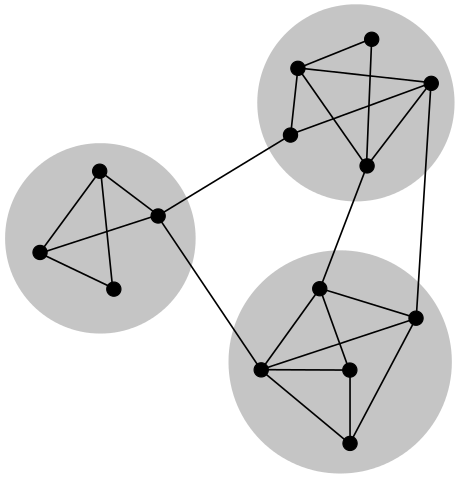
\includegraphics[width=0.3\textwidth]{graph-community-structure}
        \caption{Ejemplo de \emph{Grafo Disperso}. (Extraido de \cite{wiki:Community_structure})}
        \label{img:graph_community_structure}
      \end{figure}

      \paragraph{}
      En la figura \ref{img:graph_community_structure} se muestra un grafo disperso, que además forma 3 comunidades (conjuntos de vértices altamente conexos entre sí). Nótese que en aquiellos casos en que el grafo posea una estructura similar al de la figura, ya no es conveniente utilizar la estrategia descrita en el párrafo anterior, puesto que al tratar de preservar la estructura del mismo, no todas las aristas tienen la misma relevancia. Esto puede entenderse de manera sencilla si al comprobar la variación del grafo al eliminar una de las aristas que conectan dos comunidades. Dicha variación estructural es significativamente mayor que la ocurrida al eliminar una arista que conecta dos vértices pertenecientes a una misma comunidad.

      \paragraph{}
      Por esta razón, distintos autores han trabajado en técnicas para tratar de mantener la estructura del nuevo grafo, lo más semejante posible a la del grafo original. Para ello, las estrategias más populares se basan en la utilización de \emph{Spanners} y \emph{Sparsifiers}, los cuales se describirán a continuación en las secciones \ref{sec:spanners} y \ref{sec:sparsifiers} respectivamente. Estas técnicas han sido ampliamente estudiadas, sin embargo, en este caso se pretende orientar la descripción de las mismas sobre el \emph{modelo en semi-streaming} del cual se habló anteriormente. En este modelo se han encontrado soluciones eficientes para \emph{grafos no dirigidos}. Por contra, para el caso de los \emph{grafos dirigidos}, la búsqueda de soluciones eficientes ante este problema continuan siendo un problema abierto.

      \subsection{Spanners}
      \label{sec:spanners}

        \paragraph{}
        Se denomina \emph{Spanner} a un determinado subgrafo que mantiene las propiedades de distancia entre todos sus vértices respecto del original con una tasa máxima de variación acotada por $\alpha$. Por tanto, se denomina \emph{$\alpha$-spanner} del grafo $G = (V, E)$ a un subgrafo $H = (V, E')$ donde $E' \subset E$, construido de tal manera que se cumpla la ecuación \eqref{eq:alpha_spanner} representando $d_G(v_{i_1},v_{i_2})$ la distancia del camino más corto entre los vértices $v_{i_1}$ y $v_{i_2}$ sobre el grafo $G$.

        \begin{equation}
        \label{eq:alpha_spanner}
          \forall v_{i_1}, v_{i_2} \in V, \ d_G(v_{i_1},v_{i_2}) \leq d_H(v_{i_1},v_{i_2}) \leq \alpha \cdot d_G(v_{i_1},v_{i_2})
        \end{equation}

        \paragraph{}
        Tal y como se indica en la ecuación \eqref{eq:alpha_spanner}, lo que se pretende acotar mediante esta estrategia es por tanto, el error a nivel de distancias entre vértices. Tal y como se puede intuir, mediante el cumplimiento de esta propiedad se soluciona el problema descrito anteriormente en grafos dispersos, dado que si se elimina el único arista que conecta dos comunidades distintas, entonces la distancia del camino más corto entre los vértices de comunidades distintas variará en gran medida, posiblemente superior a la acotada por el valor $\alpha$.

        \paragraph{}
        Para la construcción de un \emph{$\alpha$-spanner} sobre el modelo en streaming existe un algoritmo sencillo que resuelve este problema para el caso del modelo de caja registradora (sección \ref{sec:streaming_cash_register}), es decir, en el cual tan solo estén permitadas adicciones. Esta estrategia se ilustra en el algoritmo \ref{code:basic_spanner}. Esta técnica es trivial y consiste en añadir únicamente al conjunto de aristas $E'$ del grafo $H$ aquellos cuya distancia del camino más corto entre sus vértices en $H$ sea mayor que $\alpha$, con lo cual se garantiza la propiedad del \emph{$\alpha$-spanner}.

        \paragraph{}
        Sin embargo, esta técnica requiere del cálculo del camino más corto entre los vértices $u$ y $v$ en cada actualización, lo cual requiere un coste de $O(card(E'))$ en tiempo, o el mantenimiento de una estructura de datos auxiliar que almacene dichas distancias, lo cual requiere de un $O(n^2)$ en espacio. El mejor resultado encontrado para este problema es la construcción de un \emph{$(2k-1)$-spanner} utilizando $O(n^(1+1/k)$ de espacio. Esta solución se ha demostrado que es óptima respecto de la precisión utilizando tan solo una pasada sobre el stream de aristas. La descripción completa de la misma se encuentra en el trabajo \emph{Streaming and Fully Dynamic Centralized Algorithms for Constructing and Maintaining Sparse Spanners} \cite{elkin2007streaming} de \emph{Elkin}.

        \paragraph{}
        \begin{algorithm}
          \SetAlgoLined
          \KwResult{$E'$ }
          $E' \gets \emptyset$\;
          \For{cada $(u, v) \in E$}{
            \If{$d_H(u,v) > \alpha$}{
              $E' \gets E' \cup \{(u,v)\}$\;
            }
          }
          \caption{Basic Spanner}
          \label{code:basic_spanner}
        \end{algorithm}

        \paragraph{}
        Para el caso general, en el cual están permitidas tanto adicciones como eliminaciones (modelo en molinete (sección \ref{sec:streaming_turnstile})) la solución básica no es trivial. El algoritmo que se describe en \cite{elkin2007streaming} se basa en la generación de árboles incrementales que se construyen a partir de la selección aleatoria de vértices. Sin embargo, esto no es sencillo cuando se permiten las eliminaciones. Por lo tanto, para la adaptación de dichas técnicas al modelo en molinete una solución es la utilización de \emph{$L_0$-Samplers}, que se describieron en la sección \ref{sec:lp_samplers}, lo cual reuquiere de múltiples pasadas sobre el stream de aristas.

        \paragraph{}
        Tal y como se ha visto en esta sección, la construcción de \emph{Spanners} añade un sobrecoste a la resolución de problemas sobre grafos, junto con una determinada tasa de error a nivel de distancias entre vértices. Sin embargo, dichos inconvenientes se ven recompensados en muchos casos por la reducción en tiempo y espacio de la resolución del problema sobre el subgrafo resultante.

      \subsection{Sparsifiers}
      \label{sec:sparsifiers}

        \paragraph{}
        Otra alternativa para la generación del subgrafo $H$ construido sobre el mismo conjunto de vértices y un subconjunto de aristas respecto del grafo $G$ son los \emph{Sparsifiers}. En este caso, en lugar de tratar de mantener la propiedad de la distancia del camino más corto entre pares de vértices, se centran en la minimización del número de cortes mínimos (eliminación de aristas) para separar el conjunto de vértices del grafo en dos subconjuntos disjuntos para cada par de vértices. A este concepto se lo denomina \emph{corte mínimo} (o \emph{Minimun Cut}) y se denota por $\lambda_{u,v}(G)$ para indicar el número de aristas a eliminar para formar dos subconjuntos disjuntos $V_{1}, V_{2}$ de tal manera que $u\in V_{1}$ y $v \in V_{2}$. Nótese por tanto que en un grafo dirigido el \emph{corte mínimo} puede tomar valores en el intervalo $[1, n\cdot(n-1)]$.  En la ecuación \eqref{eq:sparsifier_cut} se muestra la definición formal de \emph{Sparsifier} donde $A$ representa todas las combinaciones de pares de vértices y $\epsilon$ la desviación máxima permitida por el \emph{Sparsifier}, de tal manera que se denota como \emph{$\epsilon$-Sparsifier}.

        \begin{figure}
          \centering
          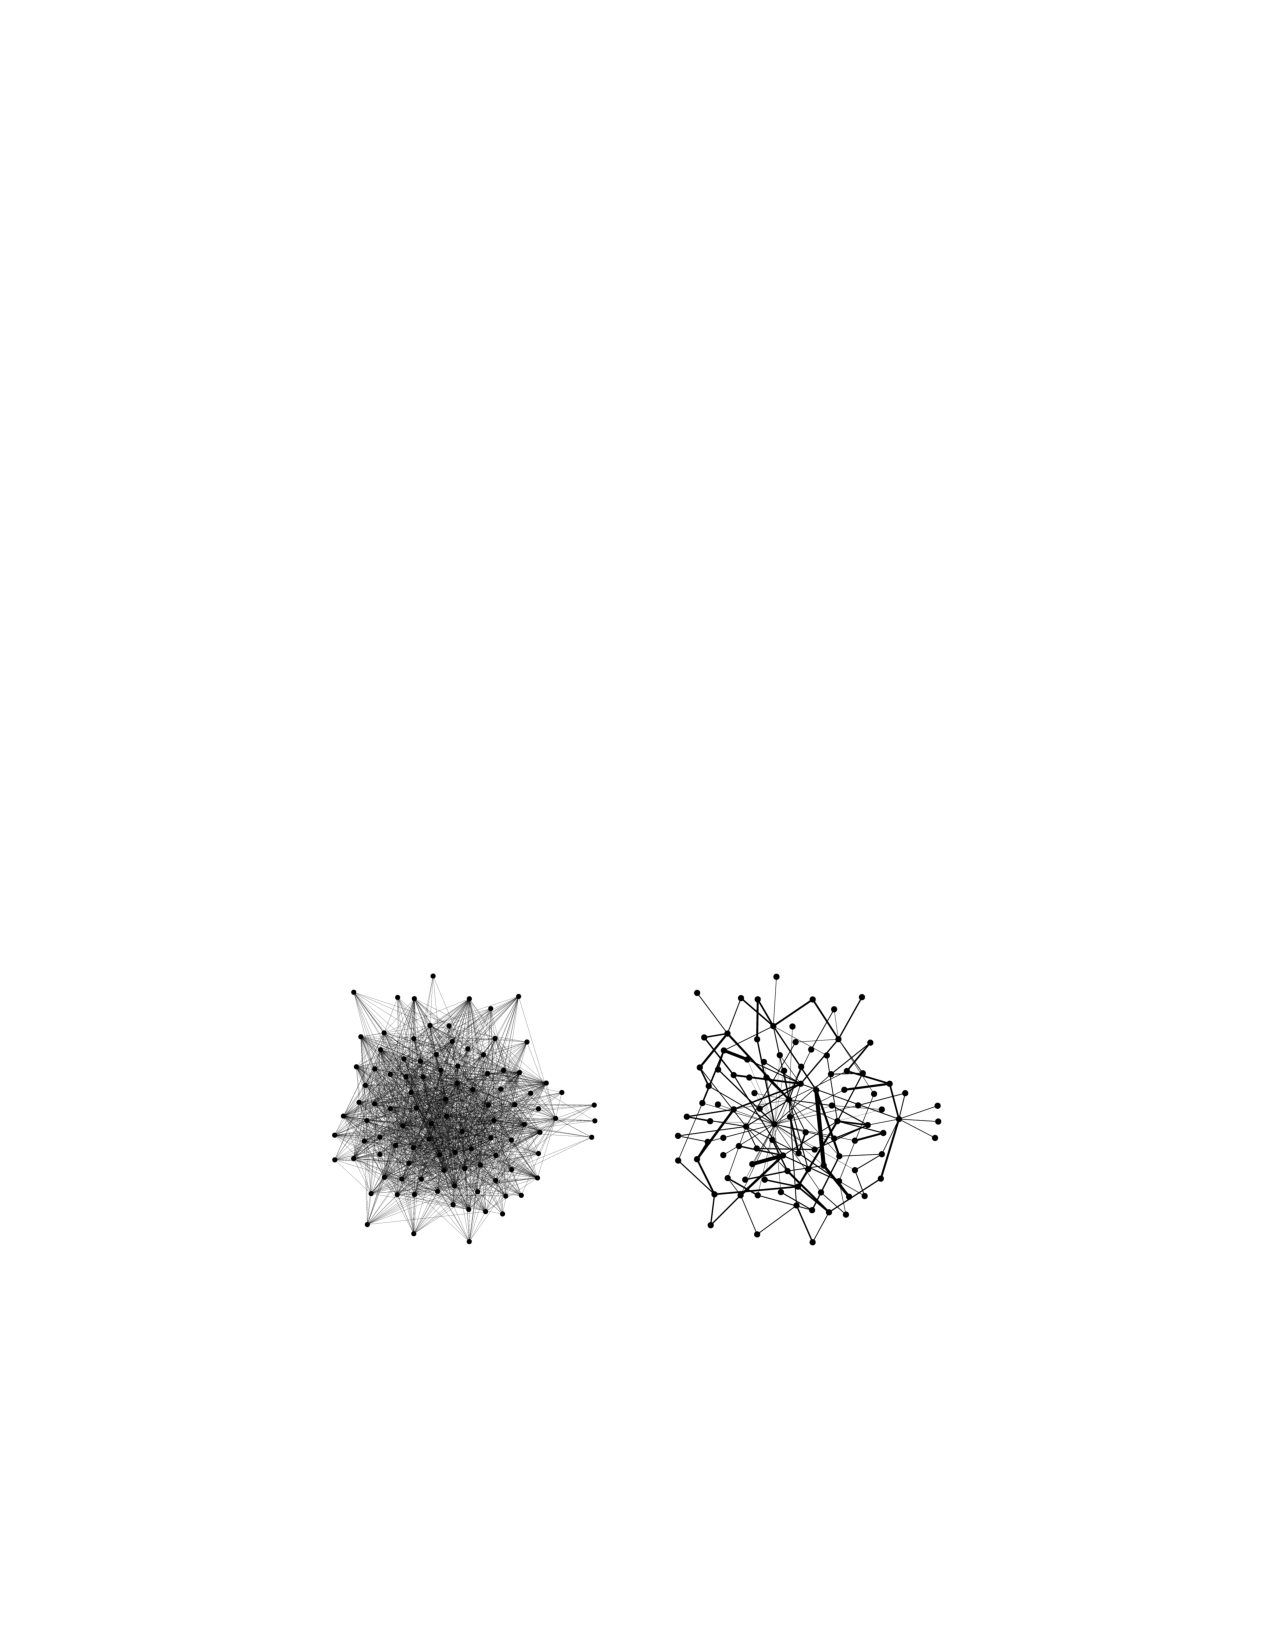
\includegraphics[width=0.5\textwidth]{graph-sparsifier}
          \caption{Ejemplo de \emph{Sparsifier}. (Extraido de \cite{harvey2011randomized})}
          \label{img:graph_community_structure}
        \end{figure}

        \begin{equation}
        \label{eq:sparsifier_cut}
          \forall A \in V \  (1-\epsilon)\lambda_A(G)\leq\lambda_A(H)\leq(1+\epsilon)\lambda_A(G)
        \end{equation}

        \paragraph{}
        A continuación se describe una definición para entender las ideas subyacentes en que se basan los \emph{Sparsifiers}. Podemos definir $G$ como $G = G_0 \subseteq G_1 \subseteq ...  \subseteq G_{i-1} \subseteq G_i \subseteq ... $ de tal manera que $Gi$ se construye eliminando los aristas de $G_{i-1}$ con probabilidad $p = 1/2$. Por tanto, $G_i$ está formado por el subconjunto de aristas de $G$ seleccionadas con probabilidad $p = (\frac{1}{2})^i$. Entonces, para construir un \emph{$\epsilon$-Sparsifier} de $G$, el valor $p$ debe ser escogido tal y como se indica en la ecuación \eqref{eq:sparsifier_p}. La demostración se encuentra en el artículo \emph{On graph problems in a semi-streaming model} \cite{feigenbaum2005graph} desarrollado por \emph{Feigenbaum y otros}. Por tanto, el problema se reduce al mantenimiento de un \emph{$L_{0}$-Sampler} que mantenga un subconjunto de aristas seleccionados con probabilidad $p$ del stream de aristas.

        \begin{equation}
        \label{eq:sparsifier_p}
          p \geq min\{6\lambda(G)^{-1}\epsilon^{-2}log(n),1\}
        \end{equation}

        \paragraph{}
        Otro enfoque diferente para la construcción de \emph{Sparsifiers} se basa en la utilización de la \emph{Matriz Laplaciana} (definida en la sección \ref{sec:laplacian_matrix}) del grafo $H$ que denotaremos como $L_{H}$. A los \emph{Sparsifiers} construidos manteniendo la propiedad definida en la ecuación \eqref{eq:sparsifier_spectral} se los denomina \emph{Spectral Sparsifiers}.

        \begin{equation}
        \label{eq:sparsifier_spectral}
          \forall x \in \mathbb{R} \  x^TL_{H}x = (1 \pm \epsilon) x^TL_{G}x
        \end{equation}


    \section{Problemas sobre Grafos}
    \label{sec:graph_problems}

      \paragraph{}
      [TODO ]

      \subsection{Matching}
      \label{sec:graph_matchings}

        \paragraph{}
        [TODO ]

      \subsection{Arbol Recubridor Mínimo}
      \label{sec:minimum_spanning_tree}

        \paragraph{}
        [TODO ]

      \subsection{Problemas de Rutado}
      \label{sec:network_routing}

        \paragraph{}
        [TODO ]

      \subsection{Problemas de Cubrimiento}
      \label{sec:network_covering}

        \paragraph{}
        [TODO ]

      \subsection{Análisis de Redes}
      \label{sec:network_analysis}

        \paragraph{}
        [TODO ]

    \section{Conclusiones}
    \label{sec:graphs_conclusions}

      \paragraph{}
      [TODO ]

\end{document}
